
\documentclass{llncs}

\usepackage{paralist}

\usepackage{amssymb, amsmath}
\usepackage{enumitem}
\usepackage{todonotes}
\usepackage{subcaption}
\captionsetup{compatibility=false}
\usepackage{url}
\usepackage{graphicx}
\usepackage{xcolor}
%\usepackage{rotating}
\usepackage{tikz}
\graphicspath{{figures/}}
\usetikzlibrary{calc,trees,positioning,arrows,chains,automata,shapes.geometric,%
    decorations.pathreplacing,decorations.pathmorphing,shapes,%
    matrix,shapes.symbols}

\usetikzlibrary{shapes,arrows,automata,positioning,calc}
\usetikzlibrary{fit,backgrounds}
\usetikzlibrary{decorations.pathreplacing}
\tikzset{
>=stealth',
  punktchain/.style={
    rectangle,
    rounded corners,
    % fill=black!10,
    draw=black, very thick,
    text width=6em,
    minimum height=3em,
    text centered,
    on chain},
  line/.style={draw, thick, <-},
  element/.style={
    tape,
    top color=white,
    bottom color=blue!50!black!60!,
    minimum width=8em,
    draw=blue!40!black!90, very thick,
    text width=10em,
    minimum height=3.5em,
    text centered,
    on chain},
  every join/.style={->, thick,shorten >=1pt},
  decoration={brace},
  tuborg/.style={decorate},
  tubnode/.style={midway, right=2pt},
}


\newcommand*\InputTable[1]{\input{tables/#1.tex}}
\newcommand*\InputTikz[1]{\input{figures/#1.tex}}
\newif\iflong
%\longtrue
\longfalse
\usepackage{marginnote}

\pagestyle{plain}

\begin{document}

\title{Mealy Machines with Timers}
\author{
Bengt Jonsson \inst{1}
\and
Frits Vaandrager \inst{2}
}
\institute{
Department of Information Technology, Uppsala University
  \and
Institute for Computing and Information Sciences, Radboud University, Nijmegen
}

\maketitle

%\begin{abstract}

%\end{abstract}

% collection of macros used in the paper

%Learners
\newcommand{\learnlib}{LearnLib}

\newcommand{\A}{{\mathcal A}}
\newcommand{\B}{{\mathcal B}}
\newcommand{\CH}{{\mathcal H}}
\newcommand{\M}{{\mathcal M}}
\newcommand{\N}{{\mathcal N}}
\newcommand{\hypoof}[2]{\mathcal{H}(#1,#2)}

\newcommand{\nat}{{\mathbb N}}
\newcommand{\integers}{{\mathbb Z}}

\newcommand{\sem}[1]{[\kern-.5mm[{#1}]\kern-.5mm]}
\newcommand{\eqclass}[1]{[{#1}]}

%DOMAIN AND RANGE
\newcommand{\dom}{{\textsf{dom}}}
\newcommand{\ran}{{\textsf{ran}}}

\newcommand{\natplus}{\nat^{>0}}
\newcommand{\realsplus}{{\mathbb R}^{\geq 0}}
\newcommand{\delays}{{\mathbb R}^{> 0}}
\newcommand{\stoptimer}{\mathit{kill}}
\newcommand{\tosymbol}{\mathit{to}}
\newcommand{\toevent}[1]{\mathit{to}[#1]}
\newcommand{\toevents}{\mbox{\sl TO}}
\newcommand{\extinputs}{\hat{I}}
\newcommand{\Head}[1]{\mathsf{Head}({#1})}
\newcommand{\Tail}[1]{\mathsf{Tail}({#1})}
\newcommand{\Last}[1]{\mathsf{Last}({#1})}
\newcommand{\expirable}{\mathit{expirable}}
\newcommand{\tvals}{\kappa}
\newcommand{\Vals}[1]{\mathit{Val}({#1})}
\newcommand{\delay}[2]{d_{[#1:#2]}}
\newcommand{\timerof}[2]{x_{#1}^{#2}}
\newcommand{\Post}{\mathsf{Post}}
\newcommand{\beh}{\mathit{beh}}
\newcommand{\untime}{\mathit{untime}}
\newcommand{\run}{\mathit{pullback}}
\newcommand{\timedword}{\mathit{tw}}
\newcommand{\timedinputword}{\mathit{tiw}}
\newcommand{\untimedinputword}{\mathit{uiw}}
\newcommand{\startedby}{\mathit{startedby}}
\newcommand{\Mealy}{\mathit{Mealy}}
\newcommand{\finitesubsets}[1]{{\mathcal{P}}_{\mathit{fin}}(#1)}
\newcommand{\conc}{\cdot}
\newcommand{\tuple}[1]{\langle #1\rangle}
\newcommand{\set}[1]{\lbrace #1\rbrace}
\newcommand{\vect}[2]{{#1}_1 , \ldots , {#1}_{#2}}
\newcommand{\setcomp}[2]{\set{#1 ~:~ #2}}
\newcommand{\domof}[1]{\dom(#1)}
\newcommand{\ranof}[1]{\ran(#1)}
\newcommand{\can}[1]{\mathit{can}({#1})}
\newcommand{\uncan}[1]{\mathit{uncan}({#1})}
\newcommand{\zone}[1]{\mathit{Zone}({#1})}
\newcommand{\vars}{\mathcal{X}}
\newcommand{\varsof}[1]{\vars(#1)}
\newcommand{\remap}{\pi}
\newcommand{\remapinst}{\rho}
\newcommand{\constr}{\phi}


\newcommand{\emptyword}{\epsilon}
\newcommand{\lengthof}[1]{|#1|}
\newcommand{\true}{{\it true}}
\newcommand{\false}{{\it false}}

%% macros for ``approximation''
\newcommand{\acttimers}{\mathit{active}}
\newcommand{\constrof}[1]{\phi_{#1}}
\newcommand{\post}{\mathit{post}}

\newcommand{\ctimers}{X}
\newcommand{\normalize}{\gamma}
\newcommand{\normalizeof}[2]{\normalize_{#2}^{#1}}
\newcommand{\timerbij}{\gamma}
\newcommand{\timerequiv}{\pi}
\newcommand{\extendedby}{\lhd}
\newcommand{\uttrace}{\textsf{tr}}
\newcommand{\uttraceof}[1]{\uttrace(#1)}
\newcommand{\uttracesof}[1]{\textsf{Tr}(#1)}
\newcommand{\strace}{\textsf{tr}_s}
\newcommand{\ssuffix}{v_s}
\newcommand{\instancesof}[1]{[\![ #1 ] \! ]}
\newcommand{\suffixbehs}[3]{({#2}^{-1}{#1})\lceil{#3}}
\newcommand{\getmemorable}[3]{\mathit{mem}_{#1,#3}(#2)}
\newcommand{\getassignment}[3]{\mathit{val}_{#1,#3,#2}}
\newcommand{\feasibleinputs}[2]{\mathit{feas}_{#2}(#1)}
\newcommand{\extend}[3]{(#1 \xrightarrow{#2/#3} \emptyset)}
\newcommand{\suffbij}[2]{g_{|#1| \to |#2|}}
\newcommand{\suftraces}{\textsf{Tr}_s}
\newcommand{\pinpof}[1]{\textit{inp}_p(#1)}
\newcommand{\sinpof}[1]{\textit{inp}_s(#1)}
\newcommand{\symbinpof}[1]{\textit{symbinp}(#1)}
\newcommand{\word}{w}
%% \newcommand{\smap}{{\cal O}}
%% \newcommand{\smappre}{{\cal O_p}}
%% \newcommand{\smapsuf}{{\cal O_s}}
%% \newcommand{\obspre}{{\cal O_U}}


\section{Introduction}
\label{sec:intro}

\marginpar{Intro still needs work}
Using active automata learning standard violations have been found in multiple implementations of
major network protocols such as TLS \cite{dRP15}, TCP \cite{FJV16} and SSH \cite{FiterauEtAl17}.
Timing often plays a crucial role in these applications but cannot be handled using existing tools.
Hence timing issues have been artificially suppressed in case studies.

There has been work on algorithms for learning timed systems, e.g., \cite{GrinchteinJL10,MensM15,CCF16},
but these approaches have complexity of these algorithms appears to be prohibitively high.
Also the specific restrictions of event recording automata sometimes make it hard to model
certain system behaviors that occur in practice.
For instance, a pattern that often occurs in protocols is that with $t$ time units after a first event $a$
there should be an event $b$, or else a timeout occurs.
% (For instance, in TCP a SYN should be followed by a SYN-ACK within a specified time interval.)
In an event recording automaton a clock is associated to each event, which is reset whenever that event occurs.
This means that upon occurrence of a second $a$ the automaton no longer remembers when the first $a$ has occurred,
and can thus not ensure the occurence of a timeout at the required moment in time.

We therefore decided to pursue a different approach. Rather than restricting the expressivity of general timed automata
until reaching a tractable model class, we explore tractable extensions of untimed automata models that appear to
be sufficiently expressive to describe the real-time behavior of practical applications.
%
Our work is inspired by recent work of Caldwell, Cardell-Oliver and French \cite{CCF16} on time delay Mealy machines.
We describe a simple variant of their model, Mealy machines with timers (MMTs), that 
(a) is able to model the timing behavior of a wide variety of communication protocols, and
(b) can be learned efficiently.
MMT's can be viewed as a formalization of the finite state machine models with countdown timers that are used by
Kurose and Ross \cite{KR13} to explain transport layer protocols.
Both time delay Mealy machines \cite{CCF16} and the event recording automata \cite{GrinchteinJL10} can not easily model such protocols.
 
Figure~\ref{fig:abp} presents a simplified model of the sender from 
the alternating-bit protocol, adapted from \cite[Figure 3.15]{KR13}.
\begin{figure}[h]
\centering
\vspace{-2 em}
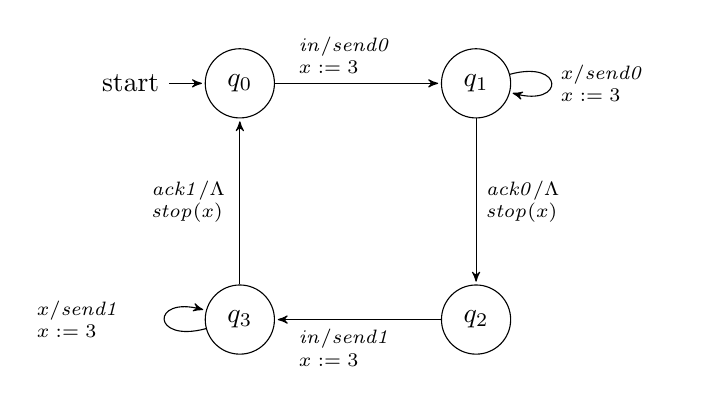
\begin{tikzpicture}[->,>=stealth',shorten >=1pt,auto,node distance=3cm,main node/.style={circle,draw,font=\sffamily\large\bfseries}]
  \node[initial, state] (1) {$q_0$};
  \node[state] (2) [right of=1] {$q_1$};
  \node[state] (3) [below of=2] {$q_2$};
  \node[state] (4) [below of=1] {$q_3$};

  \path[every node/.style={font=\sffamily\scriptsize}]
    (1) edge [text width=1.5cm] node {$\mathit{in}/\mathit{send0}$ \\ $x := 3$} (2)
    (2) edge [text width=1.5cm] node {$\mathit{ack0}/\Lambda$ \\ $\mathit{stop}(x)$} (3)
        edge [loop right, text width=1.5cm] node {$\toevent{x}/\mathit{send0}$\\ $x := 3$ } (2)
    (3) edge [text width=1.5cm] node {$\mathit{in}/\mathit{send1}$ \\ $x := 3$} (4)
    (4) edge [text width=1cm] node {$\mathit{ack1}/\Lambda$ \\ $\mathit{stop}(x)$} (1)
        edge [loop left, text width=1.5cm] node {$\toevent{x}/\mathit{send1}$\\ $x := 3$} (4);
\end{tikzpicture}
\caption{Mealy machine with a timer for alternating-bit protocol sender}
\label{fig:abp}
\end{figure}
In the diagram we write $x :=3$ to denote that a transition (re)starts a timer $x$ with value $3$,
and we write $\mathit{stop}(x)$ if s transition stops timer $x$.
For readability we have omitted trivial self-loops.
\iflong
$\Lambda$ denotes the absence of an observable output. 

In the model, input $\mathit{in}$ corresponds to a request from the upper layer to transmit data.
Initially, upon receipt of such a request, the sender builds a packet from the data and a sequence number $0$,
sends the packet over the network (output $\mathit{send0}$), and starts the timer with timeout value $3$.
If the sender receives an acknowledgement with the right sequence number $0$ (input $\mathit{ack0}$) 
then it stops the timer and jumps to state $q_2$.
Acknowledgement with the incorrect sequence number (input $\mathit{ack1}$) are ignored.
If no $\mathit{ack0}$ input arrives within $3$ timeunits, a timeout occurs and the same packet is sent again.
The behavior in states $q_2$ and state $q_3$ is analogous to that in states $q_0$ and $q_1$, respectively,
with the roles of $0$ and $1$ swapped.
\fi

The remainder of this article is structured as follows.
In Section 2, we present the formal definition of MMTs and their timed semantics.
Our timed semantics records at which (real) times inputs and outputs may occur, but we cannot observe whether some timer is started
in response to an input. Since we assume that a timeout immediately triggers an observable output, we may observe
(indirectly) the occurrence of a timeout, but we cannot observe which timer times out.
In Section 3, we present a surprising result, namely that under certain assumptions the timed semantics is equivalent to an untimed
semantics in which we can infer, for each timeout event, which previous event caused this timeout.
Intuitively, causality of timeouts can be inferred since a slight change in the timing of an input event leads to a corresponding slight change in
the timing of any timeouts that it induces.
Section 4, we use some basic concepts from the theory of timed automata (zones and DBMs) to show how we can compute the set of timers that may
timeout following some untimed run.
Section 5 presents our learning algorithm for MMTs. The equivalence of the timed and the untimed semantics allows us to prove
a Myhill-Nerode theorem for MMTs, which provides the basis for our learning algorithm. Our algorithm uses a learning algorithm for
(untimed) Mealy machines as a subroutine.
Section 6 contains some concluding remarks and lists topics for future research.


\section{Mealy Machines with One Timer}

Before we present the general model of Mealy machines with timers, we first discuss the special case of
Mealy machines with a single timer (MM1T). 
\marginnote{For multiple timers definition of semantics becomes more involved, and learning algorithm
becomes considerably more difficult.}
These are just regular (deterministic) Mealy machines,
augmented with a timeout event and a function $\tau$ that specifies how transitions affect the timer.

\begin{definition}
\label{MM1T}
A \emph{Mealy machine with one timer (MM1T)} is defined as a tuple $\M = (I, O, Q, q_0, \delta, \lambda, \tau)$, where
\begin{itemize}
\item
$I$ is a finite set of inputs, containing a special timeout event $\mathit{to}$,
\item
$O$ is a finite set of outputs, containing a special default output $\Lambda$,
\item
$Q$ is a finite set of states,
\item
$q_0 \in Q$ is the initial state,
\item
$\delta: Q \times I \rightarrow Q$ is a transition function, 
\item
$\lambda: Q \times I \rightarrow O$ is an output function, 
\item
$\tau : Q \times I \rightarrow (\nat^{>0} \cup \{ \infty, \perp \})$ is a timer function.
\end{itemize}
\marginnote{Add initial timer value?}
Function $\tau$ specifies the effect on the timer when an input $i$ occurs in state $q$.
When $\tau(q,i) \in\nat^{>0}$ then we say that input $i$ \emph{starts} the timer in state $q$,
when $\tau(q,i) = \infty$ then $i$ \emph{stops} the timer, and
when $\tau(q,i) = \perp$ then $i$ \emph{does not affect} the timer.
We require that, for each state $q$, $\tau(q,\mathit{to}) \neq\perp$, that is, 
a timeout event either starts or stops the timer.

Suppose $\delta(q,i) = q'$ and $\lambda(q,i)= o$.
Then we write $q \xrightarrow{i/o,n} q'$ if $\tau(q,i) =n \in \nat^{>0} \cup \{ \infty \}$, 
and $q \xrightarrow{i/o} q'$ or $q \xrightarrow{i/o, \perp} q'$ if $\tau(q,i) = \perp$.
\end{definition}

\begin{example}
%As a first running example, 
The MM1T of Figure~\ref{fig:abp} presents a simplified model of the sender from 
the alternating-bit protocol, adapted from \cite[Figure 3.15]{KR13}.
\begin{figure}[h]
\centering
\vspace{-2 em}
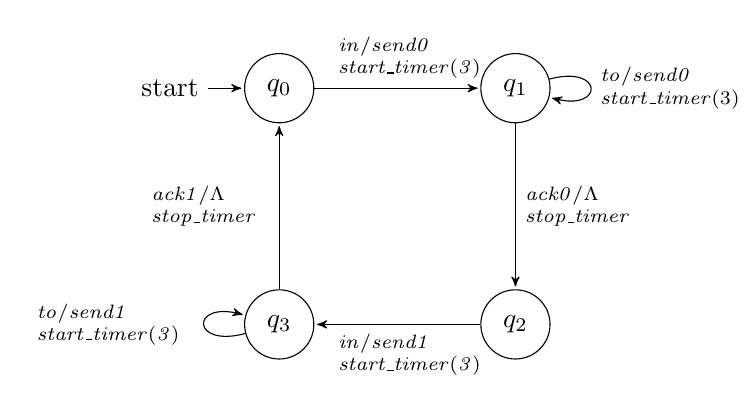
\begin{tikzpicture}[->,>=stealth',shorten >=1pt,auto,node distance=3cm,main node/.style={circle,draw,font=\sffamily\large\bfseries}]
  \node[initial, state] (1) {$q_0$};
  \node[state] (2) [right of=1] {$q_1$};
  \node[state] (3) [below of=2] {$q_2$};
  \node[state] (4) [below of=1] {$q_3$};

  \path[every node/.style={font=\sffamily\scriptsize}]
    (1) edge [text width=1.5cm] node {$\mathit{in}/\mathit{send0}$ \\ $\mathit{start\_timer(3)}$} (2)
    (2) edge [text width=1.5cm] node {$\mathit{ack0}/\Lambda$ \\ $\mathit{stop\_timer}$} (3)
        edge [loop right, text width=1.5cm] node {$\mathit{to}/\mathit{send0}$\\ $\mathit{start\_timer}(3)$ } (2)
    (3) edge [text width=1.5cm] node {$\mathit{in}/\mathit{send1}$ \\ $\mathit{start\_timer(3)}$} (4)
    (4) edge [text width=1.5cm] node {$\mathit{ack1}/\Lambda$ \\ $\mathit{stop\_timer}$} (1)
        edge [loop left, text width=2cm] node {$\mathit{to}/\mathit{send1}$\\ $\mathit{start\_timer(3)}$} (4);
\end{tikzpicture}
\caption{MM1T model of alternating-bit protocol sender}
\label{fig:abp}
\end{figure}
In the diagram we write $\mathit{start\_timer(n)}$ on a transition if this transition starts the
timer with value $n \in\nat^{>0}$, and we write $\mathit{stop\_timer}$ if the transition stops the timer.
We omit trivial self-loops: if some state $q$ does not have an outgoing $i$-transition in the diagram
then implicitly there is a transition $q \xrightarrow{i/\Lambda} q$.

In the model, input $\mathit{in}$ corresponds to a request from the upper layer to transmit data.
Initially, upon receipt of such a request, the sender builds a packet from the data and a sequence number $0$,
sends the packet over the network (output $\mathit{send0}$), and starts the timer with timeout value $3$.
If the sender receives an acknowledgement with the right sequence number $0$ (input $\mathit{ack0}$) 
then it stops the timer and jumps to state $q_2$.
Acknowledgement with the incorrect sequence number (input $\mathit{ack1}$) are ignored.
If no $\mathit{ack0}$ input arrives within $3$ timeunits, a timeout occurs and the same packet is sent again.
The behavior in states $q_2$ and state $q_3$ is analogous to that in states $q_0$ and $q_1$, respectively,
with the roles of sequence numbers $0$ and $1$ swapped.
\end{example}

\paragraph{Semantics.}
We give two semantics for MM1Ts, an untimed and a timed one.

Functions $\delta$, $\lambda$ and $\tau$ are extended to sequences of inputs in the usual way.
We define, for all $q \in Q$, $i \in I$ and $\sigma \in I^{\ast}$:
\begin{eqnarray*}
\delta(q, \epsilon) = q & , & \delta (q, i \; \sigma) = \delta(\delta(q,i), \sigma),\\
\lambda(q, \epsilon) = \epsilon & ,& \lambda(q, i \;\sigma) = \lambda(q,i) \; \lambda(\delta(q,i),\sigma),\\
\tau(q, \epsilon) = \epsilon &, & \tau(q, i \;\sigma) = \tau(q,i) \; \tau(\delta(q,i),\sigma).
\end{eqnarray*}
The untimed semantics of a MM1T $\M$ is given by the function $U_{\M}$ that assigns to each input sequence $\sigma \in I^{\ast}$
the pair $U_{\M}(\sigma) = (\lambda(q_0, \sigma), \tau(q_0, \sigma))$.
MM1Ts $\M$ and $\N$ are \emph{untimed equivalent}, written $\M \approx_{\mathit{untimed}} \N$, iff $U_{\M} = U_{\N}$.
%
Let $\sigma = i_1 \cdots i_k \in I^{\ast}$,
$\lambda(q_0, \sigma) = o_1 \cdots o_k$, and
$\tau(q_0, \sigma) = n_1 \cdots n_k$.
Then we say the sequence $i_1 o_1 n_1 i_2 o_2 n_2 \cdots i_k o_k n_k$ is a \emph{trace} of $\M$.
It is easy to see that $\M$ and $\N$ are untimed equivalent iff they have the same traces.

The timed semantics, which is slightly more involved, describes the real-time behavior of a MM1RT.
This semantics is defined by associating an infinite state transition system to a MM1T that describes all possible
configurations and transitions between them.
A \emph{configuration} of a MM1T is a pair $(q,t)$, where $q \in Q$ is a state and $t \in \bbbr^{\geq 0} \cup \{\infty\}$ 
specifies the value of the timer. We refer to the pair $(q_0, \infty)$ as the \emph{initial configuration}.
If $t = \infty$ then we say that the timer has been \emph{stopped}, otherwise it is \emph{running}.
Using four rules we define a transition relation that describes how one configuration may evolve into another.
For all $q, q' \in Q$, $i \in I$, $o \in O$, $t \in \bbbr^{\geq 0} \cup \{\infty\}$, $d \in \bbbr^{>0}$, and
$n \in \nat^{>0} \cup \{ \infty \}$,
\[
\frac{d \leq t}{(q,t) \xrightarrow{d} (q,t-d)} \hspace{1em}
\frac{q \xrightarrow{\mathit{to}/o,n} q'}{(q,0) \xrightarrow{\mathit{to}/o} (q',n)} \hspace{1em}
\frac{i \neq \mathit{to} ,~  q \xrightarrow{i/o,n} q'}{(q,t) \xrightarrow{i/o} (q',n)} \hspace{1em}
\frac{q\xrightarrow{i/o} q'}{(q,t) \xrightarrow{i/o} (q',t)}
\]
The first rule states that the value of the timer decreases when time advances, and
time can advance as long as the value of the timer is nonzero.
Here we use the convention that $\infty - d = \infty$, for any $d \in \bbbr$. This implies that when the
timer has been stopped time may advance indefinitely.
The second rule says that a timeout event occurs as soon as the timer has reached value $0$.
The third rule describes the transitions in response to a regular input, which may either start or stop the timer,
and the fourth rule describe transitions in which the timer is not affected.
A \emph{timed word} over inputs $I$ and outputs $O$ is a sequence $w = (i_0, o_0, t_0), (i_1, o_1, t_1) \cdots (i_k, o_k, t_k)$, where each $i_j \in I$, each $o_j \in O$, and each $t_j \in \bbbr^{\geq 0}$.
For a timed word $w = (i_0, o_0, t_0), (i_1, o_1, t_1) \cdots (i_k, o_k, t_k)$, a \emph{run} of MM1T $\M$ over $w$ is
a sequence 
\begin{eqnarray*}
\alpha & = & C_0 \xrightarrow{t_0} C'_0 \xrightarrow{i_0/o_0} C_1 \xrightarrow{t_1} C'_1 \xrightarrow{i_1/o_1} C_2 \cdots
\xrightarrow{t_k} C'_k \xrightarrow{i_k/o_k} C_{k+1}
\end{eqnarray*}
of transitions of $\M$ such that each $C_j, C'_j$ is a configuration of $\M$ and $C_0$ is the initial configuration.
Note that, since MM1Ts are deterministic, for each timed word $w$ there exists at most one run over $w$.
We say $w$ is a timed word of $\M$ if there exists a run of $\M$ over $w$.
Two MM1Ts $\M$ and $\N$ with the same sets of inputs are \emph{timed equivalent}, denoted $\M \approx_{\mathit{timed}} \N$, iff 
they have the same sets of observations.

\paragraph{Note}
The timed semantics is an idealization of the behavior of a real SUT: in a real system an input/output
interaction will always take a bit of time and will thus not be instantaneous.
This issue will be discussed in more detail in Section XX.
Note that a MM1T can be viewed as a very restricted type of timed automaton.

Although the definitions are quite different, it turns out that timed and untimed equivalence are almost the same.

\begin{theorem}
\label{untimedimpliestimed}
$\M \approx_{\mathit{untimed}} \N$
implies
$\M \approx_{\mathit{timed}} \N$.
\end{theorem}
\begin{proof}
Assume $\M \approx_{\mathit{untimed}} \N$ and assume
$w = (i_0, o_0, t_0), (i_1, o_1, t_1) \cdots (i_k, o_k, t_k)$ is an observation of $\M$.
Since $\approx_{\mathit{untimed}}$ is symmetric, it suffices to prove that $w$ is an observation of $\N$.

Because $w$ is an observation of $\M$, $\M$ has a run over $w$:
\[
C_0 \xrightarrow{t_0} C'_0 \xrightarrow{i_0/o_0} C_1 \xrightarrow{t_1} C'_1 \xrightarrow{i_1/o_1} C_2 \cdots
\xrightarrow{t_k} C'_k \xrightarrow{i_k/o_k} C_{k+1}
\]
Let $C_j = (q_j, u_i)$ and $C'_j = (q_j, u'_j)$, for all $j$.
Then $\M$ has a corresponding sequence of transitions:
\[
q_0 \xrightarrow{i_0/o_0, n_0} q_1 \xrightarrow{i_1/o_1, n_1} \cdots \xrightarrow{i_k/o_k, n_k} q_{k+1} .
\]
Let $\sigma = i_0 \cdots i_k$. Since $\M \approx_{\mathit{untimed}} \N$, $U_\M (\sigma) = U_\N (\sigma)$.
Therefore, $\N$ has a sequence of transitions:
\[
r_0 \xrightarrow{i_0/o_0, n_0} r_1 \xrightarrow{i_1/o_1, n_1} \cdots \xrightarrow{i_k/o_k, n_k} r_{k+1} .
\]
with all $r_j$ states of $\N$ and $r_0$ the initial state of $\N$. 
Let $D_j = (r_j, u_i)$ and $D'_j = (r_j, u'_j)$, for all $j$.
Then it is routine to check that
\[
D_0 \xrightarrow{t_0} D'_0 \xrightarrow{i_0/o_0} D_1 \xrightarrow{t_1} D'_1 \xrightarrow{i_1/o_1} D_2 \cdots
\xrightarrow{t_k} D'_k \xrightarrow{i_k/o_k} D_{k+1}
\]
is a run over $w$ of $\N$.
Thus $w$ is an observation of $\N$, as required.
\end{proof}

The converse of the implication of Theorem~\ref{untimedimpliestimed} does not hold, due to two technical problems.
The first problem is that in the timed semantics there can never be a timeout
in configurations where the timer is stopped, whereas in the untimed semantics a timeout is possible in every state.
The second problem is that in configurations where the timer is stopped, there is no observable difference between transitions that stop the timer and transitions that do not affect the timer.
In order to deal with these problems, we introduce the subclass of well-formed MM1Ts.
We show that
(a) for every MM1T there is a well-formed MM1T that is timed equivalent to it, and
(b) on well-formed MM1Ts the timed and the untimed semantics agree.

A MM1T is \emph{well-formed} if there exists a function $\mathit{timer}: Q \rightarrow \{ \mathit{on}, \mathit{off} \}$
such that:
\begin{enumerate}
\item
$\mathit{timer}(q_0) =  \mathit{off}$,
\item
if $q \xrightarrow{i/o, n} q'$ and $n \in \nat^{>0}$ then $\mathit{timer}(q') = \mathit{on}$,
\item
if $\mathit{timer}(q) =  \mathit{off}$ then $q \xrightarrow{\mathit{to}, \Lambda} q$,
\item
if $q \xrightarrow{i/o, \infty} q'$ then $\mathit{timer}(q) = \mathit{on}$ and $\mathit{timer}(q') = \mathit{off}$, and
\item
if $q \xrightarrow{i/o} q'$ then $\mathit{timer}(q)= \mathit{timer}(q')$.
\end{enumerate}

\begin{theorem}
For every MM1T $\M$ there exists a well-formed MM1T $\N$ with at most twice as many states such that 
$\M \approx_{\mathit{timed}} \N$.
\end{theorem}
\begin{proof}
Let $\M = (I, O, Q, q_0, \delta, \lambda, \tau)$ be a MM1T. 
We construct a well-formed MM1T $\N= (I, O, Q', q'_0, \delta', \lambda', \tau')$ that is timed equivalent to $\M$ 
by adding an extra bit to the state that records whether the timer is switched on or off.
We define $Q' = Q \times \{ \mathit{true}, \mathit{false} \}$ and $q'_0 = (q_0, \mathit{false})$.
Functions $\delta'$, $\lambda'$ and $\tau'$ are defined by the following five rules,
for all $q, q' \in Q$, $i \in I$, $o \in O$, $n \in \nat^{>0}$, and $b \in \{ \mathit{true}, \mathit{false} \}$,
\[
\frac{q \xrightarrow{i/o, n} q' ,~ i = \mathit{to} \Rightarrow b = \mathit{true}}
{(q,b) \xrightarrow{i/o, n} (q', \mathit{true})} \hspace{2em}
(q, \mathit{false}) \xrightarrow {\mathit{to}, \Lambda} (q, \mathit{false})
\]
\[
\frac{q \xrightarrow{i/o, \infty} q'}{(q, \mathit{true}) \xrightarrow{i/o, \infty} (q', \mathit{false})} \hspace{1em}
\frac{q \xrightarrow{i/o, \infty} q'}{(q, \mathit{false}) \xrightarrow{i/o} (q', \mathit{false})} \hspace{1 em}
\frac{q \xrightarrow{i/o} q'}{(q, b) \xrightarrow{i/o} (q', b)}
\]
The behavior of $\M$ and $\N$ is the same,
except that all $\mathit{to}$-transitions from states where the timer is off are replaced by trivial self loops (second rule),
and all transitions that stop the timer when it is already off are replaced by transitions that do not affect the timer (fourth rule).
It is straightforward to check that MM1T $\N$ is well-formed (by using
the $\mathit{timer}$ function that projects each state $(q, b)$ to its second component $b$)
and has twice as many states as $\M$.

In order to show that $\M \approx_{\mathit{timed}} \N$, we define a bisimulation relation between $\M$ and $\N$.
Let $R$ be the relation between configurations of $\M$ and $\N$ defined by:
\begin{eqnarray*}
R & = & \{ ((q,t), ((q, \mathit{true}), t)) \mid q \in Q,~ t \in \bbbr^{\geq 0} \} \cup\\
& & \{ ((q,\infty), ((q, \mathit{false}), \infty)) \mid q \in Q \}.
\end{eqnarray*}
Via a routine case distinction one can check that $R$ is a (strong) bisimulation relation between the infinite 
state transition systems associated to $\M$ and $\N$.
Clearly, strong bisimularity of transition systems implies equility of their sets of observations.
\end{proof}

Suppose that $\M = (I, O, Q, q_0, \delta, \lambda, \tau)$ is a well-formed MM1T and suppose that
$\beta = i_0 o_0 n_0 i_1 o_1 n_1 \cdots i_k o_k n_k$ is a trace of $\M$.
Then, by inspection of trace $\beta$, we can figure out whether the timer is on or off
after input sequence $\sigma = i_0 \cdots i_k$.
Define the value $\mathit{timer}(\beta) \in \{ \mathit{true}, \mathit{false} \}$ recursively as follows:
If $k=0$ then $\mathit{timer}(\beta) = \mathit{false}$. If $k > 0$ then
\begin{eqnarray*}
\mathit{timer}(\beta) & = & \left\{ \begin{array}{ll} 
\mathit{true} & \mbox{if } n_k \in\nat\\
\mathit{false} & \mbox{if } n_k = \infty\\
\mathit{timer}(\beta') & \mbox{if } n_k = \perp
\end{array}\right.
\end{eqnarray*}
with $\beta' = i_1 o_1 n_1 i_2 o_2 n_2 \cdots i_{k-1} o_{k-1} n_{k-1}$.
%
The following lemma is easy to prove by induction on the length of $\beta$:
\begin{lemma}
\label{timer lemma}
$\mathit{timer}(\beta) = \mathit{timer}(\delta(q_0, \sigma))$.
\end{lemma}

We call trace $\beta$ \emph{realizable} if no timeouts occur when the timer is off, that is,
for all $l < k$,
\begin{eqnarray*}
i_{l+1} = \mathit{to} & \Rightarrow & \mathit{timer} (i_1 o_1 n_1 i_2 o_2 n_2 \cdots i_l o_l n_l) = \mathit{true}
\end{eqnarray*}

For each realizable trace $\beta$ we may construct a corresponding run (thence the qualification ``realizable'')
\begin{eqnarray*}
\alpha & = & C_0 \xrightarrow{t_0} C'_0 \xrightarrow{i_0/o_0} C_1 \xrightarrow{t_1} C'_1 \xrightarrow{i_1/o_1} C_2 \cdots
\xrightarrow{t_k} C'_k \xrightarrow{i_k/o_k} C_{k+1}
\end{eqnarray*}
We call run $\alpha$ \emph{eager} if each transition is taken as soon as it is enabled, that is,
$i_j \neq \mathit{to} \Rightarrow t_j = 0$.
Then, in fact, for each realizable trace $\beta$ there is a unique eager run that corresponds to it.
If $\alpha$ is eager then the value $u_j$ of the timer in configuration $C_j$ is given by $u_0 = \infty$ and, for $j>0$,
\begin{eqnarray*}
u_j & = & \left\{ \begin{array}{ll} 
n_{j-1} & \mbox{if } n_{j-1} \in \nat^{>0} \cup \{\infty\}\\
u_{j-1} & \mbox{otherwise}
\end{array} \right.
\end{eqnarray*}
If $\alpha$ is eager then the timed word $w$ that corresponds to it is the sequence
$w = (i_0, o_0, t_0), (i_1, o_1, t_1) \cdots (i_k, o_k, t_k)$,
where, for all $j$,
\begin{eqnarray*}
t_j & = & \left\{ \begin{array}{ll} 
u_j & \mbox{if } i_j = \mathit{to}\\
0   & \mbox{otherwise}
\end{array}\right.
\end{eqnarray*}
Note that trace $\beta$ contains all the information required to compute $w$.

If $\beta$ is a trace of a well-formed MM1T and we insert a triple ``$\mathit{to} \; \Lambda\; \perp$'' at a point where 
the timer is off, then the result will again be a trace of the MM1T.
In fact, any trace from a MM1T can be obtained from a realizable trace by repeating this operation a number of times.
This implies the following lemma:

\begin{lemma}
\label{realizable}
Let $\M$ and $\N$ be well-formed MM1Ts with the same realizable traces.
Then  $\M \approx_{\mathit{untimed}} \N$.
\end{lemma}

\begin{theorem}
Let $\M$ and $\N$ be well-formed MM1Ts.
Then  $\M \approx_{\mathit{timed}} \N$ implies $\M \approx_{\mathit{untimed}} \N$.
\end{theorem}
\begin{proof}
Suppose $\M \approx_{\mathit{timed}} \N$. 

By Lemma~\ref{realizable}, it suffices to prove that $\M$ and $\N$ have the same realizable traces.
Let $\beta$ be a realizable trace of $\M$.
We prove by induction on the length of $\beta$ that $\beta$ is a realizable trace of $\N$ (the other inclusion follows by symmetry).

The base case is trivial, since the empty trace is a realizable trace of $\N$.

Now suppose the length of $\beta$ is $3(k+1)$, for some $k$.
Let $\beta = \gamma \; i \; o \; n$.
Then $\gamma$ is the prefix of $\beta$ of length $3 k$.
Since $\gamma$ is a realizable trace of $\M$, by induction hypothesis, $\gamma$ is a realizable trace of $\N$.
Let $\alpha$ and $\alpha'$ be the unique eager runs that correspond to $\gamma$ in $\M$ and $\N$, respectively.
Then both $\alpha$ and $\alpha'$ have the same timed word $w$. 
Let $q$ and $q'$ be the final states of $\alpha$ and $\alpha'$, respectively.
By Lemma~\ref{timer lemma}, either the timer is on both in $q$ and $q'$, or the timer is off in both $q$ and $q'$.
Moreover, in the final configurations of both runs the timers have the same value $t$.

If the last input $i$ from trace $\beta$ is different from $\mathit{to}$, then
$w \; (i \; o \; 0)$ is a timed word of $\M$.
Since $\M \approx_{\mathit{timed}} \N$, $w \; (i \; o \; 0)$ is also a timed word of $\N$.
Hence $\N$ has a realizable trace $\beta' \; i \; o \; n'$, and it remains to show $n = n'$.
We consider three cases:
\begin{enumerate}
\item
If $n = \infty$, then $\M$ has timed words $w \; (i \; o \; 0) \; (i \; o' \; d)$, for some output $o'$ and for any $d \in\bbbr^{\geq 0}$.
By well-formedness, the timer is on in state $q$, and thus it is also on in state $q'$.
Since $\N$ has the same timed words as $\M$, and since the timer is off in $q'$, we may conclude $n' = \infty$.
\item
If the timer is off in $q$ and $n = \perp$, then $\M$ has timed words $w \; (i \; o \; 0) \; (i \; o' \; d)$, for some output $o'$ and for any $d \in\bbbr^{\geq 0}$.
Since $\N$ has the same timed words as $\M$, since the timer is off in $q'$, 
and since $\N$ is well-formed, we may conclude $n' = \perp$.
\item 
If the timer is on in $q$ and $n = \perp$, then $\M$ has a timed word $w \; (i \; o \; \frac{1}{2}) \; (\mathit{to} \; o' \; t- \frac{1}{2})$, for some output $o'$.
Since $\N$ has the same timed words as $\M$, and since the value of the timer in state $q'$ is $t$, we may conclude $n' = \perp$.
\item
If $n \in \nat^{\geq 0}$, then $\M$ has a timed word $w \; (i \; o \; \frac{1}{2}) \; (\mathit{to} \; o' \; n)$, for some output $o'$.
Since $\N$ has the same timed words as $\M$, and since the value of the timer in state $q'$ is $t$, we may conclude $n' = n$.
\end{enumerate}
If the last input $i$ from trace $\beta$ equals $\mathit{to}$, then
$w \; (\mathit{to} \; o \; t)$ is a timed word of $\M$.
Since $\M \approx_{\mathit{timed}} \N$, $w \; (\mathit{to} \; o \; t)$ is also a timed word of $\N$.
Hence $\N$ has a realizable trace $\beta' \; \mathit{to} \; o \; n'$, and it remains to show $n = n'$.
By Definition~\ref{MM1T}, a timeout event either starts or stops the timer, and thus it suffices to consider the
following two cases:
\begin{enumerate}
\item
If $n = \infty$, then $\M$ has timed words $w \; (i \; o \; 0) \; (i \; o' \; d)$, for some output $o'$ and for any $d \in\bbbr^{\geq 0}$.
By well-formedness, the timer is on in state $q$, and thus it is also on in state $q'$.
Since $\N$ has the same timed words as $\M$, and since the timer is off in $q'$, we may conclude $n' = \infty$.
\end{enumerate}
\end{proof}

%\newcommand{\natplus}{\nat^{>0}}
%\newcommand{\realsplus}{\bbbr^{\geq 0}}
%\newcommand{\stoptimer}{\mathit{kill}}
%\newcommand{\tosymbol}{\mathit{to}}
%\newcommand{\toevent}[1]{\mathit{to}[#1]}
%\newcommand{\toevents}{\mbox{\sl TO}}
%\newcommand{\extinputs}{\hat{I}}
\newcommand{\acttimers}{\mathit{active}}
%\newcommand{\expirable}{\mathit{expirable}}
%\newcommand{\tvals}{\kappa}
%\newcommand{\delay}[2]{t_{[#1:#2]}}
%\newcommand{\timerof}[2]{x_{#1}^{#2}}
\newcommand{\constrof}[1]{\phi_{#1}}
\newcommand{\post}{\mathit{post}}

%\newcommand{\conc}{\cdot}
%\newcommand{\tuple}[1]{\langle #1\rangle}
%\newcommand{\set}[1]{\lbrace #1\rbrace}
%\newcommand{\vect}[2]{{#1}_1 , \ldots , {#1}_{#2}}
%\newcommand{\setcomp}[2]{\set{#1 ~:~ #2}}
%\newcommand{\domof}[1]{\dom(#1)}
%\newcommand{\ranof}[1]{\ran(#1)}
%\newcommand{\vars}{\mathcal{X}}
%\newcommand{\varsof}[1]{\vars(#1)}
\newcommand{\ctimers}{X}
%\newcommand{\remap}{\pi}
%\newcommand{\remapinst}{\rho}
\newcommand{\normalize}{\gamma}
\newcommand{\normalizeof}[2]{\normalize_{#2}^{#1}}
\newcommand{\timerbij}{\gamma}
\newcommand{\timerequiv}{\pi}
\newcommand{\extendedby}{\lhd}
\newcommand{\uttrace}{\textsf{tr}}
\newcommand{\uttraceof}[1]{\uttrace(#1)}
\newcommand{\uttracesof}[1]{\textsf{Tr}(#1)}
\newcommand{\strace}{\textsf{tr}_s}
\newcommand{\ssuffix}{v_s}
\newcommand{\suftraces}{\textsf{Tr}_s}
\newcommand{\pinpof}[1]{\textit{inp}_p(#1)}
\newcommand{\sinpof}[1]{\textit{inp}_s(#1)}
\newcommand{\symbinpof}[1]{\textit{symbinp}(#1)}
\newcommand{\word}{w}
\newcommand{\smap}{{\cal O}}
\newcommand{\smappre}{{\cal O_p}}
\newcommand{\smapsuf}{{\cal O_s}}
\newcommand{\obspre}{{\cal O_U}}

\section{General Treatment for Arbitrary Number of Timers}

It is now time to consider the general case of
Mealy machines with an arbitrary number of timers (MMnT). 
These just generalize MM1Ts in that they have a set of timers that
can be manipulated in the same way as the timer of a MM1T.
We assume an unbounded set $X$ of {\em timers};
we use $x$, $x_1$, $x_2$, etc.\ to range over timers.
Let $\toevents$ be the set of {\em timeout events} of form
$\toevent{x}$ for $x \in X$.
For a set $I$, let $\extinputs$ be $I \cup \toevents$.

\begin{definition}
\label{def:MMnT}
A \emph{Mealy machine with timers (MMnT)} is a tuple
\\
$\M = (I, O, Q, q_0, \vars, \delta, \lambda, \remap)$, where
\begin{itemize}
\item
  $I$ is a finite set of inputs,
\item
$O$ is a finite set of outputs, containing a special default output $\Lambda$,
\item
$Q$ is a finite set of states,
\item
$q_0 \in Q$ is the initial state,
\item
  $\vars$ maps each state $q \in Q$ to a finite set
$\varsof{q}$ of timers,
\item
$\delta: Q \times \extinputs \rightarrow Q$ is a transition function, 
\item
$\lambda: Q \times \extinputs \rightarrow O$ is an output function, 
\item
  $\remap$ maps each $q \in Q$ and $i \in \extinputs$ to an injective mapping from
  $\varsof{\delta(q,i)}$ to $(\varsof{q} \cup \nat^{>0})$, where also
  $y \not\in \ran(\remap(q,i))$ if $i$ is $\toevent{y}$ for timer $y$
\end{itemize}
\end{definition}
The mapping $\remap$ specifies how timers are affected when an input or timeout event $i$ occurs in state $q$.
Consider a timer $x \in \varsof{\delta(q,i)}$ in the state reached after
supplying $i$.
If $\remap(q,i)(x) \in\nat^{>0}$ then we say that $i$ \emph{starts} the timer $x$ in state $q$ and sets the timer to $\remap(q,i)(x)$.
If $\remap(q,i)(x)$ is a timer $y$ in $\varsof{q}$, then $i$ does not
affect the timer $y$, it is merely renamed to timer $x$.
If timer $y \in \varsof{q}$ is not in the range of $\remap(q,i)$, then
input $i$ \emph{kills} the timer $y$ (before it has expired).
The renaming of timers is included in order to make MMnTs independent of
actual names of timers. Two MMnTs which differ only in the names
of their timers can be made equivalent by suitable renaming of their
timers. Renaming also allows two states that differ only by the names
of their timers to be identified: this is crucial for the construction of
canonical MMnTs. The renaming of timers is analogous to the renaming of
registers in~\cite{CasselHJS16}.

%% We require that, for each state $q$, $\tau(q,\mathit{to}_x)(x) \neq\perp$, that is, when $x$ times out then $x$ is either started or stopped.


\paragraph{Note:}
Definition~\ref{def:MMnT}
does not reflect that a timeout event $\toevent{x}$ can
occur in state $q$ only if $x \in \varsof{q}$. In future updates, we  should
refine the definition to make this clear. Later in the paper (when we
derive canonical MMnTs), we will also
make sure that $\toevent{x}$ is considered if and only if $\toevent{x}$ can
actually occur in $q$ in some actual behavior.
%% if $\remap$ maps
%% $(q,i)$ to the partial function $\nu$ from timers to 
%% $\nat^{>0} \cup \{ \stoptimer \}$. If the domain of $\nu$ is empty,
%% we write $q \xrightarrow{i/o} q'$

%% The above definition of MMnT does not define any canonical form, for
%% two reasons.
%% \begin{itemize}
%% \item
%%   Wheter or not a timeout event $\toevent{x}$ can arrive in a certain state
%%   $q$ depends, in general, not only on $q$, but also on the previous
%%   sequence of events and their timing.
%% \item
%%   Equivalent MMnTs may differ only by the names of their timers.
%% \end{itemize}
%% We will later present a modified definition of a canonical form of MMnT,
%% which addresses these two problems. For now, let us ignore them and
%% get on with the definition of the semantics of MMnTs.

\paragraph{Semantics.}
We give two semantics for MMnTs, an untimed and a timed one. Let us
first consider the untimed semantics.

Suppose $\delta(q,i) = q'$ and $\lambda(q,i)= o$.
Then we write $q \xrightarrow{i/o,\remap(q,i)} q'$.
A \emph{trace} of $\M$ is a sequence of
triples
$\tuple{i_1,o_1,\remapinst_1}\tuple{i_2,o_2,\remapinst_2}
\cdots\tuple{i_n,o_n,\remapinst_n}$ such that there is a sequence 
\[
q_0 \xrightarrow{i_1/o_1,\remapinst_1} q_1
\xrightarrow{i_2/o_2,\remapinst_2}
\cdots
q_{n-1} \xrightarrow{i_n/o_n,\remapinst_n} q_n
\]
of $\M$.
Note that the set of timers $\varsof{q_j}$ can be obtained from the trace,
since it is the same as $\domof{\remapinst_j}$.
We would, intuitively, like to let the untimed semantics of $\M$ be the set
of its traces. However, it would then depend heavily on the names of
timers. Therefore, we define a normalization operation on traces, which
renames timers to canonical names. This definition is found in
Section XXX.

The timed semantics, which is slightly more involved, describes the real-time behavior of a MMnT.
This semantics is defined by associating an infinite state transition system to a MMnT that describes all possible
configurations and transitions between them.
A \emph{configuration} of a MMnT is a pair $(q,\tvals)$, where $q \in Q$ is a state and $\tvals : \varsof{q} \rightarrow \realsplus$ 
specifies the values of the timers of $q$. The initial configuration is
the pair $(q_0, \tvals_0)$, where $\tvals_0$ is the empty function.
%% If $t = \stoptimer$ then we say that the timer has been \emph{stopped}, otherwise it is \emph{running}.
Using three rules we define a transition relation that describes how one configuration may evolve into another.

For a partial function $\tvals$ from $X$ to $\realsplus$, define
%% \begin{itemize}
%% \item
  $\tvals - d$ as the function mapping each $x \in \domof{\tvals}$ to $\tvals(x) - d$.
%% \item
%%   $\tvals \setminus x$ as the function obtained from $\tvals$ by removing $x$ from the
%%   domain,
%% \item
%%   $\nu(\tvals)$ as the function obtained by applying $\nu$ to the mapping $\tvals$,
%%   i.e.,
%%   \begin{itemize}
%%     \item
%%   $\domof{\nu(\tvals)} = (\domof{\nu} \cup \domof{\tvals}) \setminus
%%   \setcomp{x}{\nu(x) = \stoptimer}$, and
%% \item
%%   $\nu(\tvals)(x) = \nu(x)$ if $\nu(x) \in \natplus$ else $\tvals(x)$.
%%   \end{itemize}
%% \end{itemize}
For all $q, q' \in Q$, $i \in I$, $o \in O$, $\tvals$ a
mapping from $\varsof{q}$ to $\realsplus$, and $d \in \realsplus$:
\[
\frac{\forall x \in \varsof{q}: \ \ d \leq \tvals(x)}{(q,\tvals) \xrightarrow{d} (q,\tvals-d)}
\quad
  \frac{\tvals(x) = 0 \quad q \xrightarrow{\toevent{x}/o,\remapinst} q'}{(q,\tvals) \xrightarrow{\toevent{x}/o} (q',\tvals\circ\remapinst)}
  \quad
  \frac{i \in I ,~  q \xrightarrow{i/o,\remapinst} q'}{(q,\tvals) \xrightarrow{i/o} (q',\tvals\circ\remapinst)}
\]
The first rule states that the value of each timer decreases when time advances, and that
time can advance as long as the values of all timers are nonzero.
The second rule says that a timeout event $\toevent{x}$ may occur
when the timer $x$ has reached value $0$.
The third rule describes the transitions in response to a regular input.
In the two last rules, the values of timers  in the successor configuration
is given by 
$\tvals\circ\remapinst$, i.e., each timer $x \in \varsof{q'}$ is either
set to a value $\remapinst(x) \in \natplus$ or takes the value of the
timer $\remapinst(x) \in \varsof{q}$ in the configuration
$(q,\tvals)$.


A \emph{timed word} over inputs $\extinputs$ and outputs $O$ is a sequence
\\
$w = (i_1, o_1, t_1), (i_2, o_2, t_2) \cdots (i_k, o_k, t_k)$, where each $i_j \in \extinputs$, each $o_j \in O$, and each $t_j \in \realsplus$.
For a timed word $w = (i_1, o_1, t_1), (i_2, o_2, t_2) \cdots (i_k, o_k, t_k)$, a \emph{run} of MM1T $\M$ over $w$ is
a sequence 
\begin{eqnarray*}
\alpha & = & C_0 \xrightarrow{t_1} C'_0 \xrightarrow{i_1/o_1} C_1 \xrightarrow{t_2} C'_1 \xrightarrow{i_2/o_2} C_2 \cdots
\xrightarrow{t_k} C'_{k-1} \xrightarrow{i_k/o_k} C_{k}
\end{eqnarray*}
of transitions of $\M$ such that each $C_j, C'_j$ is a configuration of $\M$ and $C_0$ is the initial configuration.
Note that, since MMnTs are deterministic (if we allow to observe the
identities of timers in timeout events),
for each timed word $w$ there exists at most one run over $w$.
We say $w$ is a timed word of $\M$ if there exists a run of $\M$ over $w$.
Two MMnTs $\M$ and $\N$ with the same sets of inputs are \emph{timed equivalent}, denoted $\M \approx_{\mathit{timed}} \N$, iff 
they have the same sets of timed words.

\paragraph{Note:}
We will assume the following semantic requirements on MMnTs. At this point,
we just formulate them informally, and leave the precise formalization to
a later section.
\begin{itemize}
\item
    {\em Timer-liveness}, which says that whenever $x \in \varsof{q}$, then
  there is a sequence of transitions from some reachable $(q,\tvals)$ to some
  transition where $x$ expires.
\item
  {\em Robustness}, which says that any sequence of transitions does not
  depend on precise timing. Roughtly, it means that we can slightly change
  some delay and still obtain the same untimed behavior.
\end{itemize}
Also, A design decision has to be made regarding priorities between timers. I.e.,
to determine what should happen when several timers reach $0$ simultaneously.
We take the point that the choice of timer is nondeterministic, and that
expiration of one timer may still leave the other timers unaffected so that
they can also expire. A consequence is that the behavior is then deterministic
only if we can observer the identity of timers. This issue will be resolved
by assuming that MMnTs are robust, which implies that wee need not consider
timed behaviors where two timers may expire at the same time.

\subsection{A Closer Look at Traces, and Nerode Equivalence}  
In this section, we will more precisely define a semantics of MMnT,
defined in terms of traces, which is canonical. We first need to look more
closely at traces.

A {\em suffix trace}
is a sequence
$\strace = \tuple{i_1,o_1,\remapinst_1}\cdots\tuple{i_n,o_n,\remapinst_n}$,
such that for $j = 1, \ldots , n$, we have $i_j \in \extinputs$, $o_j \in O$ and
$\remapinst_j: X \rightarrow (X \cup \natplus)$ is a mapping from timers to
timers and natural numbers, such that 
$\ranof{\remapinst_j} \subseteq (\domof{\remapinst_{j-1}} \cup \natplus)$ and
$y \not\in \ran(\remapinst_j)$ if $i_j$ is $\toevent{y}$ for
$j = 2, \ldots, n$. Define
$\domof{\strace} = \domof{\remapinst_n}$ and
  $\ranof{\strace} = \ranof{\remapinst_1}$.
For two suffix traces 
$\strace = \tuple{i_1,o_1,\remapinst_1}\cdots\tuple{i_n,o_n,\remapinst_n}$ and
$\strace' = \tuple{i_1,o_1,\remapinst_1'}\cdots\tuple{i_n,o_n,\remapinst_n'}$
with the same sequences of (extended) inputs and outputs, which
are consistent (i.e., $\remapinst_j$ and $\remapinst_j'$ agree on the intersection of their domains), we define 
$\strace \sqcup \strace' = \tuple{i_1,o_1,\remapinst_1 \cup \remapinst_1'}\cdots\tuple{i_n,o_n,\remapinst_n\cup\remapinst_n'}$.

A {\em trace} is a suffix trace $\uttrace$ with $\ranof{\uttrace} = \natplus$.

We would, intuitively, like to let the untimed semantics of $\M$ be the set
of its traces. However, it would then depend heavily on the names of
timers. Therefore, we define a normalization operation on traces, which
renames timers to canonical names.
Intuitively, a timer which is set to $p$ at the $j$th element of the trace
(i.e., in response to input $i_j$) is given the name $\timerof jp$.
A trace is normalized by consistently renaming timers in this way.
More precisly, 
consider a trace 
$\uttrace = \tuple{i_1,o_1,\remapinst_1}\cdots\tuple{i_n,o_n,\remapinst_n}$.
%% For a mapping $\remapinst_k$ and timer $x \in \domof{\remapinst_k}$, let
%% $j$ be the element in $\uttrace$ where $x$ is set, and let $p$ be the
%% value that it is set to.
%% More precisely, let $\remapinst_{[j:k]}$ denote
%% $\remapinst_j \circ \remapinst_{j+1} \circ \cdots \circ \remapinst_k$.
For $k=1, \ldots , n$,
define the injective mapping $\normalizeof{\uttrace}{k}$ on $\domof{\remapinst_k}$ by
$\normalizeof{\uttrace}{k}(x) = \timerof jp$, where 
$j$, $p \in \natplus$ are such that
$(\remapinst_j \circ \remapinst_{j+1} \circ \cdots \circ \remapinst_k)(x) = p$.
%% $\remapinst_{[j:k]}(x) = m$.
Let $\normalizeof{\uttrace}{0}$ be the empty mapping.
Then the normalization of trace
$\tuple{i_1,o_1,\remapinst_1}\cdots\tuple{i_n,o_n,\remapinst_n}$ is
the trace
\[
\tuple{i_1,o_1,(\normalizeof{\uttrace}{0} \circ \remapinst_1 \circ (\normalizeof{\uttrace}{1})^{-1})}\cdots
\tuple{\normalizeof{\uttrace}{n-1}(i_n),o_n,(\normalizeof{\uttrace}{n-1} \circ \remapinst_n \circ (\normalizeof{\uttrace}{n})^{-1})}
,
\]
where $\normalizeof{\uttrace}{k-1}(\toevent{x}) = \toevent{\normalizeof{\uttrace}{k-1}(x)}$ and
$\normalizeof{\uttrace}{k-1}(i) = i$ for $i \in I$.
%% For a trace $\uttrace = \tuple{i_1,o_1,\remapinst_1}\cdots\tuple{i_n,o_n,\remapinst_n}$ we let $\remapinst_{\uttrace}$ denote $\remapinst_n$.

Let $\uttracesof{\M}$ denote the set of normalized traces of $\M$.
The untimed semantics of a MMnT $\M$ is the set of its normalized traces.

This untimed semantics can also be used to define a Nerode equivalence on
MMnTs.

For a suffix trace $\strace$ and a bijection $\timerbij$ on $X$ let
$\timerbij(\strace)$ denote the result of renaming timers in $\uttrace$
according to $\timerbij$.
Extend $\timerbij$ to sets of traces in the natural way.
Let $X_A, X_B$ be finite sets of timers
For a bijection $\timerequiv: X_A \rightarrow X_B$, let
$\timerequiv \extendedby\timerbij$ denote that $\timerequiv$ is the restriction
of $\timerbij$ to $X_A$.

Let $\uttrace$ and $\uttrace'$ be two normalized traces of $\M$.  Define the
following adaptation of the Nerode congruence.
Let $\uttrace \equiv^{\timerequiv} \uttrace'$ denote that
$\timerequiv: \domof{\uttrace} \rightarrow \domof{\uttrace'}$ is a bijection
such that there is a bijection $\timerbij$ on $X$ with
$\timerequiv \extendedby\timerbij$ such that
\[
\uttrace\conc \strace \in \uttracesof{\M}
\qquad \mbox{if and only if} \qquad
\uttrace'\conc \timerequiv(\strace) \in \uttracesof{\M}
\]
Let $\uttrace \equiv_{\M} \uttrace'$ denote that 
$\uttrace \equiv^{\timerequiv} \uttrace'$ for some bijection
$\timerequiv: \domof{\uttrace} \rightarrow \domof{\uttrace'}$.
The equivalence $\equiv_{\M}$ can now be used to minimize $\M$, define
canonical forms, equivalence between MMnTs, etc., using standard techniques
(see, e.g.,~\cite{LeeY96}).
We would also want to use it as a basis for an automata learning algorithm.

\section{Automata Learning for MMnTs}
In this section, we present an algorithm for automata learning for MMnTs.
It is based on the Nerode equivalence $\equiv_{\M}$, which is used to adapt
the standard paradigm for automata learing, using $L^*$, which is also adapted
to register automata in~\cite{CasselHJS16}. 

Thus, two tasks must be accomplised in order to design the algorithm.
\begin{itemize}
  \item
    One task is to infer untimed traces of am MMnT.
    This is done by supplying membership queries, in the form of inputs
    with specific timing.
\item
  One task is to define suitable approximations of $\equiv_\M$, which are
  based on finite sets of suffixes. We must determine how to define suitable
  finite sets of suffix traces, which are used to define overapproximations
  of $\equiv_\M$.
\end{itemize}
We assume that we can observe
exact timing of events and that we can observe whenever a timeout event
happens. We cannot directly observe the setting of timers, or the identity
of the timer in a timeout event. However, whenever a timeout event, we
can infer where it was set, by supplying a small sequence of membership queries
with slightly perturbed timing. This is a consequence of the fact that we
assume MMnTs to be robust, implying that we can always include ``slack'' in
the timing of inputs. The normalized name of the timer follows after inferring
in which transition it was set.

Let us begin with the second task.
Intuitively, we are looking for a mechanism for characterizing a finite
set of suffixes, so that we can adapt the definition of
$\uttrace \equiv^{\timerequiv} \uttrace'$ to consider specific subsets of
suffixes. The natural way to do this is, like~\cite{Nie03}, to define
finite sets of input sequences. In our setting, a complication is that
input sequences include timer events, of form $\toevent{x}$, and that
after different traces, timer events with different timers may or may
not be enabled. We solve this complication by omitting the
identity of the timer $x$ in input sequences that characterize suffixes.

Let an \emph{input prefix} be a sequence of extended inputs.
For a trace $\uttrace$, let $\pinpof{\uttrace}$ be the sequence of its
inputs an timer events.
Let a \emph{timeout symbol} be of form $\tosymbol$, i.e., a
timer event without any clock.
Let an \emph{input suffix} be a sequence of inputs and timeout symbols.
For a suffix trace $\strace$, let $\sinpof{\strace}$ be the sequence
of inputs and timeout symbols in $\strace$, i.e., $\sinpof{\strace}$ is the
sequence of extended inputs, but with timers removed from timer events.

A central mechanism in our active learning algorithm is a procedure which
takes  an input prefix $u$ and an input suffix $v$ and return the set of
untimed traces of form $\uttrace\conc\strace$ such that
$\pinpof{\uttrace} = u$ and $\sinpof{\strace} = v$. We must here take into
consideration that we may not be able to observe all timer settings of the
SUT; only those timer settings that can actually expire sometime during
$\uttrace\conc\strace$ can actually be observed.
This may further depend on the timing of transitions
in $\uttrace\conc\strace$.

%% Let us now consider the issue that timeout events are not always
%% enabled.
%% Consider a trace $u$ of $\M$, and assume that timer $x$ is set in the
%% $i$th event of $u$. Then, in each state the corresponding timeout even
%% $\toevent{x}$ may or may not be enabled; this may
%% further depend on the timing of events in $u$, including
%% the timing of events that precede the $i$th event.
%% This motivates the following definitions.

Motivated by these considerations,
let $\uttrace = \tuple{i_1,o_1,\remapinst_1}\cdots\tuple{i_n,o_n,\remapinst_n}$.
We say that $\uttrace$ is {\em feasible} if 
there is a corresponding timed word
$\tword = (i_1, o_1, t_1) \cdots (i_n, o_n, t_n)$ for some $\vect tn$.
We then say that $\tword$ is {\em derived} from $\uttrace$.
Let $\expirable(\uttrace)$ be the set of timers $x$ such that
$\tuple{i_1,o_1,\remapinst_1}\cdots\tuple{i_n,o_n,\remapinst_n}
\tuple{\toevent{x},o_{n+1},\remapinst_{n+1}}$
is feasible for some $o_{n+1}$, $\remapinst_{n+1}$.
For $u = \pinpof{\uttrace}$ we say that $u$ is feasible iff $\uttrace$ is
feasible, and define $\expirable(u) = \expirable(\uttrace)$.

%% For a sequence $u = i_1 \cdots i_n$, define $\uttraceof{u}$ as the normalized
%% trace $\tuple{i_1,o_1,\remapinst_1}\cdots\tuple{i_n,o_n,\remapinst_n}$
%% if it exists, otherwise $\uttraceof{u} = \bot$. We say that $u$ is {\em feasible}
%% if $\uttraceof{u}$ is defined and is feasible. Define
%% $\expirable(u)$ to be $\expirable(\uttraceof{u})$.
%% It follows that $u = i_1 \cdots i_n$ is feasible if and only if whenever
%% $i_k$ is a timeout event $\toevent{x}$ for some $k$ with $1 < k \leq n$, then
%% $x \in \expirable(i_1 \cdots i_{k-1})$.
%% We will later present a technique for inferring the set $\expirable(u)$.

\paragraph{Membership Queries}
The procedure for inferring untimed traces will utilize membership queries.
We will slightly adapt the notion of membership query to make it convenient
in our current setting.

A {\em membership query} is an alternating sequence
$t_1i_2t_2i_2 \cdots t_ni_nt_{n+1}$ of delays and inputs in $\extinputs$.
The response to a membership query is either
\begin{itemize}
\item
  a sequence $o_1 o_2 \cdots o_n$ of outputs in $O$, meaning that there is
  a corresponding timed word $(i_1, o_1, t_1) \cdots (i_n, o_n, t_n)(i_{n+1}, o_{n+1}, t_{n+1})$ for some $i_{n+1}$, $o_{n+1}$, $t_{n+1}'$ with $t_{n+1} \leq t_{n+1}'$,
  or
\item
  a timeout event after some prefix $t_1i_2t_2i_2 \cdots t_{k-1}i_{k-1}t_{k}'$
  where $k \leq n+1$ and $t_k' \leq t_k$, implying that  there is
  a corresonding timed word $(i_1, o_1, t_1) \cdots (\toevent{x}, o_k, t_k')$
  for some timer $x$. By the assumption of robustness, it is easy to
  determine where the timer $x$ was set. Therefore the response to the
  membership query is the index $k$ and the normalized timer name
  $\timerof jp$, or
\item
  a {\em missing timer event} after some prefix
  $t_1i_2t_2i_2 \cdots t_{k-1}i_{k-1}t_{k}$, implying that input $i_k$, of
  form $\toevent{x}$, does not occur at the intended time.
\end{itemize}

\paragraph{Inferring traces}
We can now present a central procedure of our learning algorithm,
which is one that 
takes a feasible input prefix $u$ and an input suffix $v$ and returns the set of
feasible (normalized) untimed traces of form $\uttrace\conc\strace$ such that
$\pinpof{\uttrace} = u$ and $\sinpof{\strace} = v$.
%% restricted to the set of timers that are in
%% $\expirable(i_1 \cdots i_{k})$ for some $k \leq n$.
We assume that names of timers are normalized.

%% Consider a trace 
%% $\tuple{i_1,o_1,\remapinst_1}\cdots\tuple{i_n,o_n,\remapinst_n}$.
%% and let 
%% $w = (i_1, o_1, t_1) \cdots (i_n, o_n, t_n)$ be a corresonding timed word.
%% We introduce the following canonical naming convention for timers.
%% A timer which is set to $p$ at transition $j$ (i.e., in response to
%% input $i_j$ is given the name $\timerof jp$. This means that
%% for a timer $\timerof jp$ we have
%% $\remapinst_j(\timerof jp) = p$, and that 
%% $\timerof jp \in \remapinst_k$ only if $j \leq k$ and $\timerof jp$ has
%% not expired at or before $i_k$, and then 
%% $\remapinst_k(\timerof jp) = \timerof jp$ if $j < k$.
%% We also extend $w$ by a delay $t_{n+1} \in \realsplus$, which intuitively
%% represents that time $t_{n+1}$ elapses after the trace; such a delay
%% may be observed only if it is not interrupted by a timeout event.


%% For each timer setting in the trace, i.e., each occurrence of
%% a timer  $x \in \domof{\remapinst_i}$ with  $\remapinst_i(x) \in \natplus$,
%% defined the constraint $\constrof{\word}$ as
%% \begin{itemize}
%% \item
%%   if $i_k$ is the timeout event $\toevent{x}$, then
%%   $\constrof{\word}$ is $\delay{i}{k}= \remapinst_i(x)$,
%% \item
%%   if the trace includes no timeout event $\toevent{x}$, then
%%   $\constrof{\word}$ is $\delay{i}{(n+1)} \leq \remapinst_i(x)$.
%% \end{itemize}
%% Define $\constrof{\word}$ as
%% the conjunction of $\constrof{\word}$ for all timer settings in the trace.

The procedure must find all ways to instantiate the timeout symbols in $v$
with actual timers to obtain a feasible instantiation of $u\conc v$, and for
each such instantiation determine the set of timers that may expire after some
prefix, and how they are manipulated.

Our procedure considers increasing prefixes $z$ of extended inputs that
instantiate some prefix of $u \conc v$. For each such prefix, it
determines the set $\expirable(z)$, the constraint $\constrof{z}$
under which $z$ can be performed without any succeeding timer event, 
the timers that are in $\expirable(z')$ for some prefix $z'$ of $z$, and
their manipulation.

The procedure performs repeated membership queries for selected values
of $\vect{t}{n+1}$, and gradually adds new timers to the word together
with constraints on $\vect{t}{n+1}$ induced by these timers.

Let $\delay{j}{k}$ denote $t_{j+1} + t_{j+2} + \cdots + t_k$.
%% This means that $\remapinst_j(\timerof jp) = p$, and that 
%% $\remapinst_l(\timerof jp) = \timerof jp$ if $j < l < k$.
%% This means that $\timerof jp \in \domof{\remapinst_l}$ iff
%% $j \leq l < k$, where $\remapinst_j(\timerof jp) = p$ and
%% $\remapinst_l(\timerof jp) = \timerof jp$ for $j < l < k$.
%% Initially, $\constrof{\word}$ is the conjunction of the constraints of form
%% $\delay{j}{k}=m$ for each $i_k$ of form is $\toevent{\timerof jp}$.

%% The procedure considers prefixes in increasing order. For each input prefix
%% $z$, it
%% \begin{itemize}
%% \item determines all timers that are in $\expirable(z)$,
%% \item gradually builds a constraint $\constrof{z}$ under which $z$ can
%%   be performed without interruption by unexpected timer events,
%% \item
%%   gradually builds the mappings $\remapinst_{z'}$ for prefixes $z'$ of $z$.
%% \end{itemize}

\medskip
\noindent{\bf Algorithm} \textsl{Infer-Traces.}
\begin{description}
\item[Input:] (normalized) feasible input prefix $u$ and input suffix $v$,
\item[Returns:] set of (normalized) traces
$\uttrace\conc\strace$ such that
$\pinpof{\uttrace} = u$ and $\sinpof{\strace} = v$, together with
  constraint $\constrof{\uttrace\conc\strace}$ on derived timed words.
\item[Initialization:]
    Let $z = \emptyword$, let $\constrof{z} = \true$;
\item[Return:]
    $\textsc{Infer-Traces}(\emptyword,\emptyword,\true)$
%%     \begin{itemize}
%% \item initialize $\vect{\remapinst}n$ by letting
%%     $\timerof jp \in \domof{\remapinst_l}$ iff $i_k$ is $\toevent{\timerof jp}$
%%     with $j \leq l < k$; let $\remapinst_j(\timerof jp) = p$ and
%%     $\remapinst_l(\timerof jp) = \timerof jp$ for $j < l < k$;
%% \item let $\constrof{\uttrace}$ be
%%     the conjunction of the constraints of form
%% $\delay{j}{k}=p$ for each $i_k$ of form $\toevent{\timerof jp}$.
%%     \end{itemize}
\end{description}
\medskip
\noindent{\bf Function} $\textsc{Infer-Traces}(z,\uttrace,\constrof{\uttrace})$;
\begin{enumerate}
\item
  let $z = i_1 \cdots i_m$;
  let $\uttrace = \tuple{i_1,o_1,\remapinst_1}\cdots\tuple{i_m,o_m,\remapinst_m}$;
\item
  {\bf for} each index $k = 1, \ldots , m$ {\bf do}:
     \qquad \textit{// find all timers in $\expirable(z)$}
  \begin{enumerate}
  \item
    find $\vect t{{m+1}}$ that maximizes $\delay{k}{(m+1)}$ given
    $\constrof{\uttrace}$;
  \item
    supply membership query $t_1i_2t_2i_2 \cdots t_mi_mt_{m+1}$;
  \item
    {\bf if} unexpected timeout $\toevent{\timerof jp}$ occurs within at most
    $t_{m+1}$ after $i_m$:
    \begin{enumerate}
    \item
      add $\timerof jp$ to $\domof{\remapinst_l}$ iff
$j \leq l \leq m$, where $\remapinst_j(\timerof jp) = p$ and
      $\remapinst_l(\timerof jp) = \timerof jp$ for $j < l \leq m$;
    \item
      Add conjunct 
      $\delay{j}{(m+1)} \leq p$ to $\constrof{\uttrace}$;
      \todobj{should it be $\delay{j}{(m+1)} < p$?}
    \item if $k \neq j$ go to (a);
    \end{enumerate}
    {\bf else} do nothing;
  \end{enumerate}
  {\bf od}
\item
  {\bf if} $\lengthof{z} = \lengthof{u} + \lengthof{v}$ {\bf return}
  $\tuple{\uttrace,\constrof{\uttrace}}$;
\item
  {\bf if} $i_{m+1} \in \extinputs$:
  \[  \textbf{return } \textsc{Infer-Traces}(zi_{m+1},\uttrace\tuple{i_{m+1},o_{m+1},\emptyset},\phi')
  \]
  where $\phi'$ is $\constrof{\uttrace}$ if $i_{m+1} \in I$, otherwise, if
  $i_{m+1} = \toevent{\timerof jp}$, it is obtained from $\constrof{\uttrace}$
  by replacing $\delay{j}{(m+1)} \leq p$ by $\delay{j}{(m+1)} = p$.
  \item
  {\bf else} \hspace*{4cm} \textit{// \ $i_{m+1}$ is the timeout symbol}
    \[
    \textbf{return} \mathop\bigcup_{\timerof jp \in \expirable(z)}
     \textsc{Infer-Traces}(z\toevent{\timerof jp},\uttrace\tuple{\toevent{\timerof jp},o_{m+1},\emptyset},\phi')
     \]
  where  $\phi_j^p$ is obtained from $\constrof{\uttrace}$
  by replacing $\delay{j}{(m+1)} \leq p$ by $\delay{j}{(m+1)} = p$.
\end{enumerate}
Intuitively, the function
$\textsc{Infer-Traces}(z,\uttrace,\constrof{\uttrace})$ finds
all timers in $\expirable(z)$ by testing for each $k$ whether 
it is possible
to set a timer at the $k$th transition that may expire after the
$m$th transition. Any such timer expiration adds a constraint to
$\constrof{\uttrace}$, which is included in the constraints used to find
further timers.
This is done by finding a timed word is found which maximises the
time within which it is able to expire, subject to the constraints under
which other, already detected, timers cannot expire. If no expiration is
observed, then it is ascertained that no such timer exists.
If such a timer may exist, then some expiration must be observed, either
by a timer set at the $k$th transition and expiring at the $m+1$st transition,
or by a so-far undetected timer that can expire because the membership
query exposes a new timing pattern. In either case, the new detected timer
is added to the word, and the procedure restarts.

\paragraph{Generating MMnTs}
Having solved the problem of inferring untimed traces, we can now
define our generalization of $L^*$, which is based on the
Nerode equivalence defined earlier
%% We can now present our algorithm for active learning of MMnTs.
%% The main structure of the algorithm is inherited from other active
%% algorithms: it builds on a Nerode equivalence, which is defined based on
%% the set of (untimed) traces of an MMnT.
%% Thus, the algorithm has two nontrivial parts.
%% \begin{itemize}
%%   \item
%%     One part is to infer untimed traces of am MMnT, essentially building
%%     a prefix tree of untimed traces. This is done by supplying membership
%%     queries, following the ideas of the previous section.
%% \item
%%   One part is to ``fold'' the prefix tree developed in the first part
%%   into a MMnt. This can be done by adapting the suitable tools for active
%%   automata learning, as found in $L^*$
%%   (adapted for Mealy machines in~\cite{Nie03} and to automata with
%%   data registers in~\cite{CasselHJS16}).
%% \end{itemize}
%% We assume that we can observe
%% exact timing of events and that we can observe whenever a timeout eMMvent
%% happens. On the other hand, we cannot observe the setting and resetting of
%% timers, and we cannot observe which timer caused an observed timeout event.


\begin{definition}[Observation Table]
  An \emph{observation table} is a tuple
  $\tuple{U,U^+,V,\smap}$, where
  \begin{itemize}
  \item $U$ is a set of (feasible) {\em input prefixes},
  \item $U^+$ is a set of {\em extended input prefixes}, each of form $ui$ for
    $i \in \extinputs$ (note that $U^+$ is in general not disjoint from $U$),
  \item
    $V$ is a set of input suffixes,
  \item
    $\smap$ maps each extended input prefix $u$ in $U^+$ and input suffix $v$
    to a set of pairs $\tuple{\uttrace,\strace}$ such that 
    $\uttrace\conc\strace$ is an untimed trace with
$\pinpof{\uttrace} = u$ and $\sinpof{\strace} = v$.
   We use $\smappre(u,v)$ for $\uttrace$ and 
   $\smapsuf(u,v)$ for $\strace$.
  \end{itemize}
\end{definition}
For an observation table and $u \in U^+$,
let $\obspre(u)$ denote
\(
\displaystyle\mathop\sqcup_{v \in V}\smappre(u,v)
\),
i.e., $\obspre(u)$ includes manipulation of all timers that may be
exposed by any of the suffixes in $V$.
The observation table defines the following equivalence
Let $u \equiv_{\smap}^{\timerequiv} u'$ denote that
$\timerequiv: \domof{\obspre(u)} \rightarrow \domof{\obspre(u')}$
is a bijection such that there is a bijection $\timerbij$ on $X$ with
$\timerequiv \extendedby\timerbij$ such that for each $v \in V$
\[
\strace \in \smapsuf(u,v)
\qquad \mbox{if and only if} \qquad
\timerequiv(\strace) \in \smapsuf(u',v)
\]
Let $u \equiv_{\smap} u'$ denote that 
$u \equiv_{\smap}^{\timerequiv} u'$ for some bijection
$\timerequiv: \domof{\obspre(u)} \rightarrow \domof{\obspre(u')}$.

Say that an observation table is {\em closed} if for each
$ui \in U^+$ there is a short prefix $u' \in U$ and a $\timerbij$ such that
$ui \equiv_{\smap}^{\timerequiv} u'$.

A closed observation table $\tuple{U,U^+,V,\smap}$ can be used to construct
a hypothesis  MMnT $\M = (I, O, Q, q_0, \vars, \delta, \lambda, \remap)$, where
\begin{itemize}
\item
  $Q = U$ and $q_0 = \emptyword$,
\item
  $\vars$ maps each state $u \in Q$ to $\domof{\obspre(u)}$,
\item
  $\delta(u,i)$ is the unique short prefix $u'$ such that
  $ui \equiv_{\smap}^{\timerequiv} u'$. If so, then
  $\remap(u,i) = \remap\circ\timerequiv^{-1}$,
  where $\remap$ is the remapping of the last transition in
  $\obspre(ui)$.
  \item
$\lambda$ is obtained easily from the work (To be done)
\end{itemize}










%% \input{../OldFiles/oldstuff-bj-nclocks}
%% \input{textbank}
\section{Learning algorithm}
In order to learn a MMTO, we may adapt a standard algorithm for learning (untimed) Mealy machines, e.g., $L^\ast$.
We assume that the learner knows an upper bound $B$ on the possible timeout values, that is, a constant $B \in \nat$ such
that, for each $q \in Q$, $\tau(q) < \infty$ implies $\tau(q) < B$.
Whenever we discover a new state, that is, a prefix $\beta$ of inputs that uniquely determines a state in the MMTO,
we may figure out the corresponding value of the timeout function as follows: by taking transitions in $\beta$ as
fast as possible, we ensure that the value of the timer is $0$ upon arrival in the state.
Now we just wait for $B$ time units. If an event occurs before the $B$ time units have elapsed, we record the delay after
which this event occurs: this is the value of the timeout function for state $\beta$.
Otherwise, if no event occurs and $B$ time units have elapsed, we know the value of the timeout function is $\infty$.
We record the observed value of the timeout function in a separate column in the observation table.
(Or, equivalently, we may annotate the output in the column for suffix $\mathit{to}$ with this value.)
Now suppose we have found a state that can be reached by a prefix $\beta$, and we want to figure out
whether the timer is reset after some input $i$.
We can do this as follows.
First we perform all the inputs from $\beta$ as fast as possible, ensuring that the value of the timer is $0$ in
the resulting state.
Now we wait $0.5$ time units.
If a timeout has occurred during this interval then we know that the timeout value of the state after $\beta$ is $0$.
Thus input $i$ may only occur at time $0$ and it does not make any difference whether or not the timer is reset as part
of an $i$-transition.
If no timeout occurs during the $0.5$ time units, then we perform the input $i$ and wait for $B$ time units.
If no timeout occurs during this interval then we conclude that the timer is switched of after trace $\beta \; i$,
and again it does not make a difference whether or not the timer is reset as part of the $i$-transition.
If, however, a timeout occurs $t$ time units after the input $i$, then there are two cases:
\begin{enumerate}
\item
$t$ is equal to the value of the timeout function for trace $\beta \; i$, and we may conclude that
the timer is reset as part of the $i$-transition, or 
\item
$t$ is equal to the value of the timeout function for trace $\beta \; i$ \emph{minus} $0.5$, and
we may conclude that the timer is not reset in the $i$-transition.
\end{enumerate}
We record the observed value of the reset function in the observation table in the entry for row $\beta$ and
column $i$.

The above algorithm can be implemented as a minor adaptation of existing implementations of $L^{\ast}$. The query
complexity is the same as that of $L^{\ast}$. The total time of running a query will be at most $(u+1) \cdot B + 0.5$,
where $u$ is the number of \emph{to} inputs that occur in the query.

\paragraph{Research questions}
Work out the proofs. What is the best/easiest way to implement this?
Does it also work for register automata.
Can we generalize these ideas to richer classes of automata (e.g. more clocks, splitting inputs and outputs into separate
transitions, closure under composition)?
Implement and apply this stuf, for instance to the TCP protocol.

\bibliographystyle{plain}
\bibliography{abbreviations,dbase}

\end{document}
